%%%% h2snn_ijcai27_v3b.tex -- IJCAI-27 version of H2S-NN, model v3-B (methodology spec v1.14)
%%%% Experiments are unfinished: every number that does not exist yet is \res.

\documentclass{article}
\pdfpagewidth=8.5in
\pdfpageheight=11in

\usepackage{ijcai27}

\usepackage{times}
\usepackage{soul}
\usepackage{url}
\usepackage[hidelinks]{hyperref}
\usepackage[utf8]{inputenc}
\usepackage[small]{caption}
\usepackage{graphicx}
\usepackage{amsmath}
\usepackage{amssymb}
\usepackage{amsthm}
\usepackage{booktabs}
\usepackage{multirow}
\usepackage[switch]{lineno}

% Comment out this line in the camera-ready submission
\linenumbers

\urlstyle{same}

\newtheorem{proposition}{Proposition}

\newcommand{\R}{\mathbb{R}}
\newcommand{\method}{\textsc{H2S-NN}}
\newcommand{\wisp}{\textsc{WISP}}
\newcommand{\norm}[1]{\left\lVert #1\right\rVert}
\newcommand{\transpose}{\mathsf{T}}
\newcommand{\concat}{\mathbin\Vert}
\newcommand{\res}{{\scriptsize[result]}}
\newcommand{\inc}{\trianglelefteq}

\pdfinfo{
/TemplateVersion (IJCAI.2027.0)
}

\title{H2S-NN: Meta-Path-Structured Sheaf Neural Networks\\ for Heterogeneous Heterophilic Graphs}

% Anonymous submission
\author{
    Anonymous submission
}

\begin{document}

\maketitle

\begin{abstract}
Heterogeneous graphs are frequently heterophilic: two papers that share an author, for example, often belong to different fields, so a connection does not imply label agreement. Existing methods split the graph into one homogeneous view per meta-path schema and fuse the views. Once the views are built, all node pairs joined under the same schema are treated alike, and the intermediate entities and the particular meta-path instances that join a pair no longer take part in propagation. We ask whether heterophily can instead be handled on the original graph, by making meta-path instances part of the structure the model operates on. We propose \method{}, a sheaf neural network in which each meta-path instance, sampled by random walks without a meta-path list, is a face of the graph's own sheaf: its restriction maps are composed from the maps of its edges, so no parameters are added, and it is coupled to every node and edge it traverses, including the intermediate ones. Instances that share an edge interact through that edge's stalk. Node, edge and face stalks form one quadratic energy whose minimiser is unique for all parameter values and gives the node representations. On twelve node-classification benchmarks and eight link-prediction tasks spanning a range of heterophily, \res{}; controlled variants on identical sampled instances show \res{}.
\end{abstract}

%======================================================================
%======================================================================
\section{Introduction}
\label{sec:introduction}

Heterogeneous graphs are a common representation for modeling complex relational structures, such as citation networks \cite{liu2014meta} or social interactions \cite{singh2025overview}. Unlike homogeneous graphs, they contain multiple types of nodes and relations with distinct semantic roles \cite{sun2013mining}. Moreover, many of them are also heterophilic, meaning that adjacent nodes may have different labels or attributes, which makes similarity-based neighbor aggregation and leads to \cite{lin2025heterophily}. A graph can be both heterogeneous and heterophilic, which means the graphs can have multiple node types while adjacent nodes have different attributes. This makes learning considerably harder than under either property alone. Because an edge joins nodes of different types, which share neither a feature space nor a label space, agreement between neighbors is not even defined and can only be examined between target-type nodes connected through other nodes. Furthermore, the nodes in between decide whether such a pair agrees. In Figure~\ref{fig:example}(a), papers P1 and P9 share the author A7 but belong to different fields, whereas a narrow subject such as S3 may link papers of one field. Methods designed for heterophily usually assume a single node type, and methods designed for heterogeneity usually assume homophily, so neither addresses both properties together.

To handle the situation where nodes of the target type are linked only through nodes of other types, meta-paths are the standard way to express how they are connected. A meta-path schema such as \texttt{Paper-Author-Paper} (PAP) describes a composite relation between two target-type nodes that neither node expresses alone \cite{sun2011pathsim}, and a meta-path instance such as P1--A7--P9 is one concrete occurrence of it. Meta-paths connect target nodes whose labels are comparable, distinguish the semantics of different relations (PAP is a shared author, PSP a shared subject), and make heterophily measurable on heterogeneous graphs \cite{lin2025heterophily}. They therefore underlie most heterogeneous graph models \cite{wang2019han,fu2020magnn,yang2023sehgnn}.

\begin{figure*}[t]
  \centering
  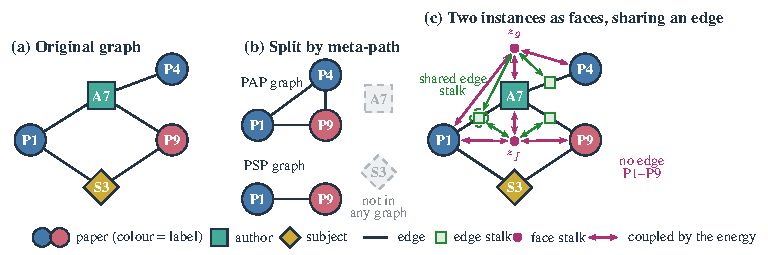
\includegraphics[width=0.92\textwidth]{figure/h2snn_example_v3b3.pdf}
  \caption{Running example. \textbf{(a)} A heterogeneous heterophilic citation graph: papers P1, P4, P9 (colour = label), author A7, subject S3. \textbf{(b)} Splitting by meta-path schema builds one paper graph per schema (PAP, PSP); A7 and S3 appear in neither. \textbf{(c)} \method{} keeps the meta-path instances P1--A7--P9 and P1--A7--P4 as faces of the original graph. Each face stalk (dots) is coupled to every node and edge of its instance, including A7, and the two faces share the stalk of the edge P1--A7 (dashed). No edge P1--P9 is added.}
  \label{fig:example}
\end{figure*}

However, existing neural networks methods for heterogeneous heterophilic graphs address heterophily and meta-paths indirectly. They decompose the graph into one view per meta-path schema and then fuse the views \cite{lu2026addressing,chen2025adaptive,li2025hetero2net,guo2023homophily,shen2025heterophily,wang2025homophily}, as shown in Figure~\ref{fig:example}(b). Propagation therefore runs on derived graphs instead of the original one instead of the original one, and node pairs that follow the same schema are distinguished only by their endpoints, so the meta-path instances that connect them, and the nodes and edges in between, are ignored. Instance encoders such as MAGNN \cite{fu2020magnn} keep the intermediate nodes but write the result only to the target node, and sheaf-based models \cite{braithwaite2024heterogeneous} use edges information alone. These gaps lead to two research questions: \textbf{RQ1}, can a single model on the original graph predict under heterophily using meta-path instances, without per-schema branches?” \textbf{RQ2}, given the same meta-path instances, does using them as structure, by coupling the nodes and edges they traverse and the instances that share an edge, improve prediction over using them as features at their endpoints?

To address these questions, we introduce the \textbf{Heterogeneous Heterophilic Sheaf Neural Network (\method{})}, which handles heterophily on the original graph and treats meta-paths as part of the structure the model operates on, not as extra input. \method{} represents each sampled meta-path instance as a two-dimensional cell (2-cell), which we call a face, attached to the nodes and edges it traverses (nodes and edges are the 0- and 1-cells). A face is never closed into a loop, so an instance does not need to return to its start. Node representations are obtained by solving one energy problem over this structure, in which a node is influenced by its edges and by every meta-path instance through it, including intermediate nodes. Instances that share an edge interact through that edge’s stalk. Each instance carries a learned weight computed from its own nodes and relations. Edges act through learned, direction-aware transformations, and each instance acts through the composition of the transformations of its edges, so neighbors of different classes need not be pulled toward the same representation. Our main contributions are summarized as follows:
\begin{enumerate}
\item We propose \method{}, a single model on the original graph that handles heterophily without per-schema branches (RQ1). Its sampler, \wisp{}, draws meta-path instances by random walks without a meta-path list, so the model without pre-defined schemas.
\item We retain each meta-path instance as a face whose maps are fixed by the maps of its edges, so that every node of the instance, including intermediate ones, is coupled to it with no added parameters (RQ2). Controlled variants on identical sampled instances is coupled to it with no added parameters, and instances that share an edge interact through its stalk (RQ2). Controlled variants on identical sampled instances test whether this coupling improves prediction.
\end{enumerate}


%======================================================================
\section{Related Work}
\label{sec:related}

\paragraph{Meta-paths for heterogeneity and heterophily.} HAN \cite{wang2019han} builds meta-path neighbours and learns attention between them, and SeHGNN \cite{yang2023sehgnn} and LMSPS \cite{li2024lmsps} aggregate over a set of schemas, the latter selecting the useful ones. Heterophily-aware models such as Hetero$^2$Net \cite{li2025hetero2net}, H2SGNN \cite{lu2026addressing} and LatGRL \cite{shen2025heterophily} build latent or induced homogeneous graphs per schema. In all of these the intermediate nodes of an instance are not part of the graph on which messages are exchanged. MAGNN \cite{fu2020magnn}, MECCH \cite{fu2024mecch} and MF2Vec \cite{kim2024mf2vec} do read the intermediate nodes and weight instances, but the encoded instance is written to the target node only. H2G-former \cite{lin2025heterophily} takes a different route: a heterogeneous attention model with $k$-hop masks on sampled subgraphs, with meta-paths entering only the heterophily measure. \method{} keeps the original graph and writes each instance back to all of its nodes and edges.

\paragraph{Sheaf and higher-order networks.} Cellular sheaves attach a vector space and learned restriction maps to a graph, so that neighbours are compared after a change of coordinates \cite{hansen2020sheaf,bodnar2022neural,barbero2022sheaf}, with cooperative and directional extensions \cite{ribeiro2026cooperative,fiorini2025sheaves}. HetSheaf \cite{braithwaite2024heterogeneous} adapts them to heterogeneous graphs through edges only. Sheaf hypergraph networks \cite{duta2023sheafhyper} couple the members of a hyperedge through a shared stalk with a freely learned map per node and hyperedge. Cell-complex and topological networks \cite{bodnar2021cwn,hajij2022tdl,hajij2025ctnn} pass messages over higher-dimensional cells without a sheaf whose face maps are fixed by the graph's own edge maps. The two differences of \method{} from a sheaf hypergraph network are that the maps of a face are composed from the maps of its edges, and that faces sharing an edge are coupled through that edge's stalk (Section~\ref{sec:energy}).

\section{Preliminaries}
\label{sec:background}

\subsection{Heterogeneous graphs and meta-paths}
 A heterogeneous graph is $G=(V,E,\phi,\psi)$ with node types $\phi:V\to\mathcal{T}$ and relation types $\psi:E\to\mathcal{R}$, where $|\mathcal{T}|>1$ or $|\mathcal{R}|>1$. We keep one edge per fact, not one per direction. A meta-path schema of length $\ell$ is a typed relation sequence $\pi: t_0\xrightarrow{r_1}t_1\cdots\xrightarrow{r_\ell}t_\ell$ \cite{sun2011pathsim}; a meta-path instance is a sequence $f=(v_0,e_1,v_1,\ldots,e_\ell,v_\ell)$ with $\phi(v_i)=t_i$ and $\psi(e_i)=r_i$. The schema is a type-level pattern, the instance is one occurrence of it. The nodes $v_1,\dots,v_{\ell-1}$ are intermediate; in Figure~\ref{fig:example}, PAP is a schema and P1--A7--P9 an instance with A7 intermediate.

\subsection{Heterophily}
 Labels are comparable only between target-type nodes, so heterophily is measured on the graphs that length-two schemas from the target type to itself induce. We report three measures, each computed with the code of its source. The $\mathcal{H}^2$ index of H2GB \cite{lin2025heterophily} is the mean over these graphs of $1-h_{\mathrm{adj}}$, where $h_{\mathrm{adj}}$ is the class-imbalance-corrected adjusted homophily \cite{platonov2023characterizing}. MLH, the label heterophily on meta-path graphs, and MDE, the meta-path-based Dirichlet energy, which measures attribute heterophily, are those of Hetero$^2$Net \cite{li2025hetero2net}.

\subsection{Sheaves on a graph and its incidence poset}
 A \emph{cell} is the generic word for a node (0-cell), an edge (1-cell) or a face (2-cell). A cellular sheaf assigns every cell a vector space, its \emph{stalk}; a vector in it is also called a stalk, and we speak of node, edge and face stalks. Every incident pair $p\inc q$ has a linear \emph{restriction map} $F_{p\inc q}$ from the stalk of $p$ to that of $q$, and maps compose along chains: $F_{e\inc f}F_{v\inc e}=F_{v\inc f}$. On a graph, only the pairs $v\inc e$ exist. Eliminating the edge stalks $s_e$ from $\sum_e\sum_{v\in e}\norm{F_{v\inc e}x_v-s_e}^2$ leaves $\tfrac12\sum_e\norm{F_{u\inc e}x_u-F_{v\inc e}x_v}^2$, which with identity maps is half the quadratic form of the graph Laplacian. We add faces through the \emph{incidence poset}: $v\inc e$ if $v$ lies on $e$, $e\inc f$ if $e$ is an edge of $f$, and $v\inc f$ if $v$ is a node of $f$. We use only this order relation and require no attaching maps as in a cell complex.

%======================================================================
\section{Methodology}
\label{sec:method}

\subsection{Problem}
Given a heterogeneous graph with type-dependent node features $x^{\mathrm{raw}}_v\in\R^{d_{\phi(v)}}$ (types without features receive a learned vector per node) and no list of meta-path schemas, we learn a predictor $p_\theta(o;G)$ for an object $o$: a target node (classification) or a typed node pair (link prediction). The parameters minimise the average of a loss $\mathcal{L}$, cross-entropy or binary cross-entropy, over labelled training objects.

\subsection{Overview}
\begin{figure*}[t]
  \centering
  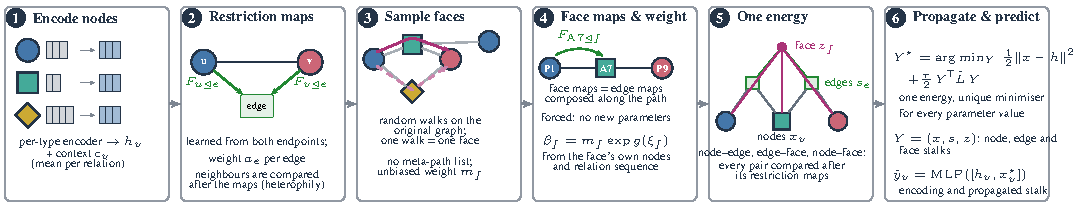
\includegraphics[width=\textwidth]{figure/h2snn_overview_v3b2.pdf}
  \caption{Overview of \method{}: (1) encode nodes, (2) learn restriction maps on edges, (3) sample faces with \wisp{}, (4) derive face maps from edge maps and weight each face, (5) combine node, edge and face stalks in one energy, (6) propagate by minimising the energy and predict.}
  \label{fig:pipeline}
\end{figure*}
We introduce \method{}, a Heterogeneous Heterophilic Sheaf Neural Network, for supervised learning on heterogeneous heterophilic graphs. As shown in Figure~\ref{fig:pipeline}, \method{} consists of six stages. First, \emph{node encoding} maps typed features into a shared stalk space. Second, \emph{restriction maps} are learned on every edge, so that neighbours are compared in the coordinates of the edge instead of the raw space and need not have similar embeddings. Third, \wisp{} samples meta-path instances by random walks as \emph{faces}, and fourth, the maps of each face are composed from the maps of its edges and the face receives a weight. Fifth, node, edge and face stalks interact through \emph{one energy}, in which a node is influenced by its edges and by every face through it, and faces that share an edge are coupled through its stalk. Finally, the node representations are obtained by minimising the energy anchored at the node encodings, and a prediction head reads them together with the encodings. Together, these stages allow \method{} to handle heterophily on the original graph and to use meta-path instances as part of its structure.

\subsection{Encoding and Restriction Maps}
Because nodes of different types must be compared by the same maps, each node is first encoded into a $d$-dimensional vector, $h_v=\operatorname{GELU}(\operatorname{LN}(W_{\phi(v)}x^{\mathrm{raw}}_v+b_{\phi(v)})+q_{\phi(v)})$ with type-specific $W,b$ and a type embedding $q$. Two nodes with similar features can play different roles, so $c_v$ adds the mean of $h$ over the neighbours of $v$ under every relation and direction.

Because neighbours under heterophily should not be forced to agree in the raw space, an edge $e=(u\xrightarrow{r}v)$ carries one learned restriction map per endpoint, and the two endpoint values are compared in the coordinates of the edge, as in sheaf neural networks \cite{hansen2020sheaf,bodnar2022neural}. Each map is orthogonal and depends on both endpoints, the relation and the role of the endpoint:
\begin{equation}
\begin{aligned}
  F_{v\inc e}&=R_{r,\rho}\,H_2(u)H_1(u),\\
  u&=\operatorname{MLP}([h_v,c_v,h_{v'},c_{v'},\zeta_r,\rho]),
\end{aligned}
  \label{eq:maps}
\end{equation}
where $v'$ is the other endpoint, $\zeta_r$ a relation embedding, $\rho$ the role, $R_{r,\rho}$ a learned rotation, and $H_1,H_2$ Householder reflections. Orthogonality keeps all compositions of maps orthogonal, and the pair conditioning lets the identity of an intermediate node enter the geometry, which relation-only maps cannot do. Each edge also has a positive weight $a_e=c_e^2$.

\subsection{Faces: Meta-Path Instances with Forced Maps}
\label{sec:wisp}
\wisp{} supplies the faces without a meta-path list. From every anchor node it draws $r$ random walks on the original graph; anchors are the nodes of the target type for node classification, the nodes of both endpoint types of the target relation for link prediction, and every node for graph classification. A walk draws its length uniformly from $\{2,\ldots,\ell_{\max}\}$, chooses uniformly among relation--direction pairs that lead to an unvisited node, then uniformly among those neighbours, and is discarded at a dead end. A walk and its reversal give one instance. Each walk $\omega$ has probability $p(\omega)$, and each instance receives the sampling weight $m_f=\sum_{\omega\to f}\frac1r\,p(\omega)/q_{\mathrm{mix}}(\omega)$, where $q_{\mathrm{mix}}$ is the distribution the walks were drawn from. The weighted sum of instance terms is then an unbiased estimate of the one defined by $p$ (Appendix~\ref{app:proofs}); this concerns the sum before normalisation (Section~\ref{sec:prop}). Training draws new walks every epoch, and evaluation uses one fixed draw shared by all compared models.

A face is one instance $f=(v_0,e_1,\ldots,v_\ell)$. It is \emph{not} closed: there is no edge between $v_0$ and $v_\ell$. A face has a stalk $z_f$, and its restriction maps are not new parameters. We fix $F_{v_0\inc f}=I$ and compose the edge maps along the path,
\begin{equation}
\begin{aligned}
  F_{e_i\inc f}&=F_{v_{i-1}\inc f}\,F_{v_{i-1}\inc e_i}^{\transpose},\\
  F_{v_i\inc f}&=F_{e_i\inc f}\,F_{v_i\inc e_i}.
\end{aligned}
\label{eq:forced}
\end{equation}
The first line states that the map into the face from edge $e_i$ sends the stalk of $e_i$ back to the frame of $v_{i-1}$ and then forward to the face; the second line carries the frame on to $v_i$. By construction $F_{e_i\inc f}F_{v_{i-1}\inc e_i}=F_{v_{i-1}\inc f}$ and $F_{e_i\inc f}F_{v_i\inc e_i}=F_{v_i\inc f}$, so all maps compose along the incidence poset.

\begin{proposition}[Forced maps]\label{prop:forced}
With Equation~\eqref{eq:forced}, node, edge and face maps form one sheaf on the incidence poset. In the energy $E$ of Equation~\eqref{eq:energy}, every face term vanishes at each configuration in which the graph's own sheaf is consistent, that is, $F_{v\inc e}x_v=s_e$ on every edge. Freely learned face maps do not have this property and in general shrink the set of zero-energy configurations.
\end{proposition}
Hence faces add no constraint where the edges already agree. This is a statement about $E$; after the normalisation of Section~\ref{sec:prop}, consistent configurations are rescaled by $D^{1/2}$, and $D$ changes when faces are added.

\subsection{One Energy}
\label{sec:energy}
The model keeps three kinds of stalks: $x_v$ for every node, $s_e$ for every edge and $z_f$ for every face, collected in $Y=(x,s,z)$. The energy asks every comparable pair of cells to agree after their restriction maps:
\begin{equation}
\begin{aligned}
  E(Y)=&\tfrac12\sum_{e}a_e\!\!\sum_{v\in e}\!\norm{F_{v\inc e}x_v-s_e}^2\\
  +&\tfrac12\sum_{f}\beta_f\Bigl[\sum_{e\in f}\norm{F_{e\inc f}s_e-z_f}^2+\!\sum_{v\in f}\norm{F_{v\inc f}x_v-z_f}^2\Bigr].
\end{aligned}
\label{eq:energy}
\end{equation}
The first sum compares each node with its edges; the second compares each face with its edges and with every one of its nodes, intermediate ones included. The weight $\beta_f=w_fm_f$ combines the sampling weight with a learned score $w_f=\exp g(\xi_f)$, where $g$ reads the encodings $h$ of all nodes of the instance and its relation embeddings, so two instances of one schema can differ in influence.

Consider the instances $f=$ P1--A7--P9 and $g=$ P1--A7--P4 of Figure~\ref{fig:example}(c), which share the edge $e=$ P1--A7. Face $f$ is compared with its three nodes and two edges, so A7 is pulled toward the common value $z_f$ together with P1 and P9. Face $g$ does the same for P1, A7, P4. Both are also compared with the single stalk $s_e$, so $f$ and $g$ constrain the same variable. Let $L=\nabla^2E$ and $D_e=2a_e+\sum_{h\ni e}\beta_h$.

\begin{proposition}[Coupling]\label{prop:reach}
(i) For every node $v$ of face $f$, the $(x_v,z_f)$ block of $L$ is $-\beta_fF_{v\inc f}^{\transpose}$, which is nonzero. (ii) For two faces $f,g$ that contain the edge $e$, eliminating $s_e$ adds to the $(z_f,z_g)$ block the coupling $-\frac{\beta_f\beta_g}{D_e}F_{e\inc f}F_{e\inc g}^{\transpose}$.
\end{proposition}
If the edge--face term is dropped, (ii) disappears: $f$ and $g$ then interact only through the nodes they share, here P1 and A7. If faces were coupled only to edges, (i) would disappear, and a node's stalk would be reached only through edges. Part (i) alone does not separate faces from the hyperedges of a sheaf hypergraph network; the forced maps of Equation~\eqref{eq:forced} and part (ii) are what does.

\subsection{Propagation as a Minimiser and Prediction}
\label{sec:prop}
Let $D$ be the block diagonal of $L$ and $\hat L=D^{-1/2}LD^{-1/2}$, so that node, edge and face stalks are on the same scale and influence does not grow with degree. Only node stalks have an input, the encoding $h$; edge and face stalks are free. The propagated stalks solve
\begin{equation}
  Y^\star=\arg\min_Y\ \tfrac12\norm{x-h}^2+\tfrac{\tau}{2}\,Y^{\transpose}\hat LY,\qquad \tau=e^{\theta},
  \label{eq:solve}
\end{equation}
that is, each node stays close to its encoding while the energy is small. $\tau$ is learned, with a larger learning rate than other parameters. The prediction is $\hat y_v=\operatorname{MLP}([x^\star_v\concat h_v])$, so a node's own encoding is not mixed with disagreeing neighbours before the nonlinear head \cite{zhu2020beyond}; link prediction scores a pair of such vectors with a decoder on the two node vectors.

The analysis involves three systems. $E$ and $L$, before normalisation, are the objects of Propositions~\ref{prop:forced} and~\ref{prop:reach} and of the sampling guarantee. $\hat L$ is the normalised system of Equation~\eqref{eq:solve}; a configuration that is consistent in $E$ has values scaled by $D^{1/2}$ in $\hat L$. $\hat S$ is obtained from $\hat L$ by eliminating the edge and face stalks exactly.
\begin{proposition}[Unique solution]\label{prop:unique}
For every parameter value, Equation~\eqref{eq:solve} has a unique minimiser, $x^\star=(I+\tau\hat S)^{-1}h$, and $\operatorname{cond}(I+\tau\hat S)\le1+\tau$.
\end{proposition}
The bound on the condition number concerns $\hat S$ only. The solver is preconditioned conjugate gradients on the system that keeps the stalks of edges lying on several faces, which gives the same $x^\star$, and the gradient is taken implicitly, so no unrolled layers are stored.

\paragraph{What this establishes for heterophily.} The node-level map $h\mapsto x^\star$ is a resolvent, the same form as personalised PageRank propagation \cite{gasteiger2019appnp}; what is new is the operator inside it. Edge and face stalks have no input features, so they carry no information beyond what the nodes supply; they change the geometry in which nodes interact. For heterophily, it can be shown that maps of the form of Equation~\eqref{eq:maps} admit configurations in which nodes of different classes are consistent in the edge coordinates without being equal (existence only; it does not imply that training finds them), a mechanism that edge-level sheaf models share. What faces add is a comparison that no edge expresses: P1 and P9 are compared \emph{through} A7 with A7's own maps, and instances sharing an edge inform each other. Whether this coupling improves prediction under heterophily is an empirical question, which we test by removing it (Section~\ref{sec:discussion}); we do not claim it from the construction.

\subsection{Variants and Cost}
\label{sec:cases}
The model contains the following configurations, which we compare on identical sampled instances. \emph{No faces}: $\beta_f=0$, an edge-sheaf model. \emph{No edge--face term}: faces are coupled only to their nodes and edge stalks are eliminated, so each edge acts as a direct term between its endpoints; with \emph{Free face maps} this is close to a sheaf hypergraph network. \emph{No node--face term}: faces are coupled only to their edges. \emph{Endpoint edge}: each face is replaced by one edge between $v_0$ and $v_\ell$ that carries the composed map and the weight $\beta_f$. \emph{Face as feature}: $\beta_f=0$ in the solve, and a weighted mean of the transported encodings of each instance is passed to the prediction head; with relation-only maps this equals the instance encoder of MAGNN, as we checked numerically. \emph{Free face maps}: the maps into the face are learned instead of forced. The weight ladder restricts $g$ to a constant (\emph{Uniform}), to the relation sequence (\emph{Schema}) or to the endpoints and relation sequence (\emph{Endpoints}); the full model additionally sees the intermediate nodes.

Edges that lie on at most one face are eliminated exactly, so the cost depends on the edges shared by several faces. On ACM, DBLP and IMDB with $d=32$, the solver converged in 9, 11 and 10 iterations at tolerance $10^{-4}$, on one RTX 4060 (8 GB) card; peak memory and time per epoch are in Table~\ref{tab:cost}. The cost does not depend on the number of schemas.

%======================================================================
\section{Experiments}
\label{sec:experiments}

\subsection{Experiment Settings}
We evaluate on node classification (main task) and link prediction; graph classification checks that the model covers the task and is reported in Appendix~\ref{app:data}.

\paragraph{Datasets.} For node classification we use four HGB benchmarks \cite{lv2021hgb}, ACM, DBLP, IMDB and Freebase (24\%/6\%/70\% splits), and eight H2GB benchmarks \cite{lin2025heterophily}: ogbn-mag, mag-year, oag-cs, oag-eng, oag-chem, IEEE-CIS-G, H-Pokec and PDNS, with their official loaders and splits; PDNS is evaluated on later time windows and is the one inductive dataset. They cover a wide range of heterophily (Table~\ref{tab:hetero}). For link prediction we use eight tasks: ACM paper--author, DBLP author--paper, IMDB movie--actor, Freebase book--book, PubMed disease--disease, LastFM user--artist, ogbn-mag paper--paper and H-Pokec user--user. The target relation is split by fact into 81\%/9\%/10\% (Freebase by unordered pair), and held-out facts are removed in both directions from the message graph and from every sampled instance. Features computed from the target relation or describing the other endpoint are removed, and a leakage audit is run before any result.

\paragraph{Baselines.} We compare with homogeneous homophilic (GCN \cite{kipf2017gcn}, GAT \cite{velickovic2018gat}, ChebNetII \cite{he2022chebnetii}), homogeneous heterophilic (NSD \cite{bodnar2022neural}, CSNN \cite{ribeiro2026cooperative}), heterogeneous homophilic (R-GCN \cite{schlichtkrull2018rgcn}, HAN \cite{wang2019han}, MAGNN \cite{fu2020magnn}, SeHGNN \cite{yang2023sehgnn}, HiNormer \cite{mao2023hinormer}, PSHGCN \cite{he2024spectral}) and heterogeneous heterophilic models (H2G-former \cite{lin2025heterophily}, Hetero$^2$Net \cite{li2025hetero2net}, H2SGNN \cite{lu2026addressing}, HetSheaf \cite{braithwaite2024heterogeneous}). Following HGB, the groups are named Hom./hom., Hom./het., Het./hom. and Het./het. by whether the graph is modeled as homogeneous or heterogeneous and the method designed for homophilic or heterophilic settings. Link prediction uses a subset covering all groups.

\paragraph{Protocol.} Node classification is scored by Macro-F1 and Micro-F1, with Macro-F1 averaged over the classes present in each split's true labels; IMDB is multi-label (binary cross-entropy per genre, threshold at logit zero, 4,573 labelled movies). For link prediction we follow the HGB protocol: each test positive is paired with one negative whose tail is a two-hop neighbour of the head within the target type, validation uses random tail negatives, and we report ROC-AUC and MRR. Every method, baselines included (HetSheaf through an adapter), is rerun under one protocol: the same optimiser, learning-rate and dropout ranges, no scheduler, epochs and early stopping on the validation metric as in each benchmark's source protocol, and the original feature preprocessing of each method. Hyperparameters are found by plain Bayesian search with 100 trials on seed 0, and the best configuration is run on seeds 0--4. For \method{} the search covers the embedding size $d$, the maximum walk length $\ell_{\max}\in\{2,\dots,5\}$ and the number of walks per anchor $r\in\{8,\dots,64\}$, besides the shared axes; the proposal distribution of \wisp{} is uniform. We report mean $\pm$ standard deviation over five seeds and test \method{} against the best other method on each dataset and metric with Welch's $t$-test (about 48 tests), reporting raw and adjusted $p$-values with the adjustment chosen after the results.

\begin{table*}[t]
  \centering
  \caption{Heterophily of the node-classification datasets, each computed with the code of its source and recomputed here: $\mathcal{H}^2$ with H2GB's code and meta-path rule, MLH and MDE with Hetero$^2$Net's code and meta-path sets (so the sets may differ between rows). Higher means more heterophilic.}
  \label{tab:hetero}
  \scriptsize
  \setlength{\tabcolsep}{3pt}
  \begin{tabular}{lcccccccccccc}
    \toprule
    & ACM & DBLP & IMDB & Freebase & ogbn-mag & mag-year & oag-cs & oag-eng & oag-chem & IEEE-CIS-G & H-Pokec & PDNS \\
    \midrule
    $\mathcal{H}^2$ & \res & \res & \res & \res & \res & \res & \res & \res & \res & \res & \res & \res \\
    MLH & \res & \res & \res & \res & \res & \res & \res & \res & \res & \res & \res & \res \\
    MDE & \res & \res & \res & \res & \res & \res & \res & \res & \res & \res & \res & \res \\
    \bottomrule
  \end{tabular}
\end{table*}

\subsection{Results}
\label{sec:results}
Table~\ref{tab:node-cls} reports node classification and Table~\ref{tab:link-pred} link prediction. \res{}

\begin{table*}[t]
  \centering
  \caption{Node classification, Macro-F1, mean $\pm$ std over five seeds (Micro-F1 in Appendix~\ref{app:data}). Best values are bold.}
  \label{tab:node-cls}
  \scriptsize
  \setlength{\tabcolsep}{2.6pt}
  \begin{tabular}{llcccccccccccc}
    \toprule
    \textbf{Group} & \textbf{Model} & ACM & DBLP & IMDB & Free. & mag & m-year & oag-cs & oag-eng & oag-chem & IEEE & Pokec & PDNS \\
    \midrule
    \multirow{3}{*}{Hom./hom.} & GCN & \res & \res & \res & \res & \res & \res & \res & \res & \res & \res & \res & \res \\
    & GAT & \res & \res & \res & \res & \res & \res & \res & \res & \res & \res & \res & \res \\
    & ChebNetII & \res & \res & \res & \res & \res & \res & \res & \res & \res & \res & \res & \res \\
    \midrule
    \multirow{2}{*}{Hom./het.} & NSD & \res & \res & \res & \res & \res & \res & \res & \res & \res & \res & \res & \res \\
    & CSNN & \res & \res & \res & \res & \res & \res & \res & \res & \res & \res & \res & \res \\
    \midrule
    \multirow{6}{*}{Het./hom.} & R-GCN & \res & \res & \res & \res & \res & \res & \res & \res & \res & \res & \res & \res \\
    & HAN & \res & \res & \res & \res & \res & \res & \res & \res & \res & \res & \res & \res \\
    & MAGNN & \res & \res & \res & \res & \res & \res & \res & \res & \res & \res & \res & \res \\
    & SeHGNN & \res & \res & \res & \res & \res & \res & \res & \res & \res & \res & \res & \res \\
    & HiNormer & \res & \res & \res & \res & \res & \res & \res & \res & \res & \res & \res & \res \\
    & PSHGCN & \res & \res & \res & \res & \res & \res & \res & \res & \res & \res & \res & \res \\
    \midrule
    \multirow{4}{*}{Het./het.} & H2G-former & \res & \res & \res & \res & \res & \res & \res & \res & \res & \res & \res & \res \\
    & Hetero$^2$Net & \res & \res & \res & \res & \res & \res & \res & \res & \res & \res & \res & \res \\
    & H2SGNN & \res & \res & \res & \res & \res & \res & \res & \res & \res & \res & \res & \res \\
    & HetSheaf & \res & \res & \res & \res & \res & \res & \res & \res & \res & \res & \res & \res \\
    \midrule
    Ours & \method{} & \res & \res & \res & \res & \res & \res & \res & \res & \res & \res & \res & \res \\
    \bottomrule
  \end{tabular}
\end{table*}

\begin{table*}[t]
  \centering
  \caption{Link prediction, ROC-AUC (MRR in Appendix~\ref{app:data}), mean over five seeds.}
  \label{tab:link-pred}
  \footnotesize
  \setlength{\tabcolsep}{4pt}
  \begin{tabular}{lcccccccc}
    \toprule
    \textbf{Model} & ACM & DBLP & IMDB & Freebase & PubMed & LastFM & ogbn-mag & H-Pokec \\
    \midrule
    GCN & \res & \res & \res & \res & \res & \res & \res & \res \\
    NSD & \res & \res & \res & \res & \res & \res & \res & \res \\
    R-GCN & \res & \res & \res & \res & \res & \res & \res & \res \\
    MAGNN & \res & \res & \res & \res & \res & \res & \res & \res \\
    HetSheaf & \res & \res & \res & \res & \res & \res & \res & \res \\
    H2G-former & \res & \res & \res & \res & \res & \res & \res & \res \\
    \midrule
    \method{} & \res & \res & \res & \res & \res & \res & \res & \res \\
    \bottomrule
  \end{tabular}
\end{table*}

%======================================================================
\section{Discussion}
\label{sec:discussion}

\subsection{What the Faces Contribute}
To separate the contribution of faces from that of weighting and capacity, the variants of Section~\ref{sec:cases} are compared on identical sampled instances, the same evaluation draw and parameter counts within 5\% (Table~\ref{tab:ablation}). \emph{Endpoint edge} tests whether the intermediate nodes matter, \emph{Face as feature} whether coupling a face to all its cells matters beyond a MAGNN-type encoding, \emph{No edge--face term} whether the shared edge stalk matters, and \emph{Free face maps} whether forcing the maps matters. The criteria are fixed before running. If the full model is not significantly better than the \emph{Endpoints} weight variant on at least two of ACM, DBLP and IMDB, we do not claim that intermediate nodes contribute through the weights. If it is not significantly better than \emph{No edge--face term}, we report that coupling faces through shared edge stalks does not by itself improve accuracy, and that the contribution is the geometry in which the face maps are forced. \res{}

\begin{table}[t]
  \centering
  \caption{Controlled variants on identical sampled instances (Macro-F1, mean over five seeds).}
  \label{tab:ablation}
  \footnotesize
  \setlength{\tabcolsep}{3pt}
  \begin{tabular}{lcccc}
    \toprule
    \textbf{Variant} & ACM & DBLP & IMDB & Freebase \\
    \midrule
    \method{} (full) & \res & \res & \res & \res \\
    No faces & \res & \res & \res & \res \\
    No edge--face term & \res & \res & \res & \res \\
    No node--face term & \res & \res & \res & \res \\
    Endpoint edge & \res & \res & \res & \res \\
    Face as feature & \res & \res & \res & \res \\
    Free face maps & \res & \res & \res & \res \\
    Uniform / Schema / Endpoints weights & \res & \res & \res & \res \\
    \bottomrule
  \end{tabular}
\end{table}

\subsection{Heterophily and Cost}
Reviewers of an earlier version asked for heterophily to be established and analysed, and for cost to be reported against graph size. We therefore report the accuracy of the full model against the baselines by $\mathcal{H}^2$ and by node degree, and time and memory per epoch with graph size (Table~\ref{tab:cost}). \res{}

\begin{table}[t]
  \centering
  \caption{Cost per epoch with graph size.}
  \label{tab:cost}
  \footnotesize
  \setlength{\tabcolsep}{4pt}
  \begin{tabular}{lccc}
    \toprule
    & ACM & DBLP & IMDB \\
    \midrule
    Time per epoch (s) & \res & \res & \res \\
    Peak memory (MB) & \res & \res & \res \\
    \bottomrule
  \end{tabular}
\end{table}

\subsection{Limitations}
Edges, faces and the energy are symmetric, so the strength of influence between two nodes is the same in both directions; the energy is quadratic and the propagation linear, so no band-pass response is built in; faces are simple walks, so branching meta-structures are not represented; and the weights scale a face but cannot change its maps, which the edges fix. Edge and face stalks have no input features. Existence results do not imply that training finds a class-separating configuration.

%======================================================================
\section{Conclusion}
We asked whether heterophily can be handled on the original heterogeneous graph by making meta-path instances part of its structure. \method{} does so by treating each sampled instance as a face of the graph's own sheaf, with maps composed from its edges, coupled to every node and edge of the instance and to other faces through shared edges, and solved together with nodes and edges in one energy with a unique minimiser. \res{}

\bibliographystyle{named}
\bibliography{references}

%======================================================================
\appendix
\section{Proofs}
\label{app:proofs}
Every edge map is orthogonal, so the maps of Equation~\eqref{eq:forced} are orthogonal and $F^{\transpose}F=I$.

\emph{Unbiased sampling.} Walks are drawn independently, $r$ per anchor, from $q_{\mathrm{mix}}$. Then $\mathbb{E}[\sum_fm_fL_f]=\sum_a r\sum_\omega q_{\mathrm{mix}}(\omega)\frac1r\frac{p(\omega)}{q_{\mathrm{mix}}(\omega)}L_{f(\omega)}=\sum_a\sum_\omega p(\omega)L_{f(\omega)}$, where $L_f$ is the part of $L$ contributed by face $f$ at unit weight.

\emph{Proposition~\ref{prop:forced}.} Composition is verified in Equation~\eqref{eq:forced}. If $F_{v\inc e}x_v=s_e$ for all incident pairs, set $z_f=x_{v_0}$; then $F_{e_i\inc f}s_{e_i}=F_{v_{i-1}\inc f}x_{v_{i-1}}=z_f$ by induction, and $F_{v_i\inc f}x_{v_i}=F_{e_i\inc f}s_{e_i}=z_f$, so every face term vanishes.

\emph{Proposition~\ref{prop:reach}.} (i) The only term of Equation~\eqref{eq:energy} containing both $x_v$ and $z_f$ is $\frac12\beta_f\norm{F_{v\inc f}x_v-z_f}^2$, giving $-\beta_fF_{v\inc f}^{\transpose}$, nonzero because $F_{v\inc f}$ is orthogonal and $\beta_f>0$. (ii) The $s_e$ block of $L$ is $D_eI$, because each of the two endpoints contributes $a_e$, each face containing $e$ contributes $\beta_h$, and the maps are orthogonal. The coupling of $s_e$ to $z_f$ is $-\beta_fF_{e\inc f}^{\transpose}$. The $(z_f,z_g)$ block of $L$ is zero, so the Schur complement with respect to $s_e$ gives $0-(-\beta_fF_{e\inc f})\,D_e^{-1}\,(-\beta_gF_{e\inc g}^{\transpose})=-\frac{\beta_f\beta_g}{D_e}F_{e\inc f}F_{e\inc g}^{\transpose}$. We also checked this numerically on random orthogonal maps.

\emph{Proposition~\ref{prop:unique}.} $L_{xx}$ is block diagonal with $D_vI$ because there are no node--node terms, so $\hat L_{xx}=I$. The block of edge and face stalks, $\hat L_{ww}$, is positive definite: its quadratic form is zero only if every $s_e$ and then every $z_f$ is zero, since $a_e,\beta_f>0$. Hence the Schur complement $\hat S=I-\hat L_{xw}\hat L_{ww}^{-1}\hat L_{wx}$ satisfies $0\preceq\hat S\preceq I$, the objective is strictly convex, $x^\star=(I+\tau\hat S)^{-1}h$, and $\operatorname{cond}(I+\tau\hat S)\le1+\tau$.

\section{Datasets, Settings and Full Results}
\label{app:data}
This appendix reports dataset statistics, the Micro-F1 and MRR tables, search spaces, graph classification and further results. Graph classification follows HetSheaf's protocol (TU MUTAG, PROTEINS, ENZYMES, NCI1 with node types taken from the label one-hot, constant features, 80/10/10 split, seeds 0--4); because node types are derived from labels, it checks generalisability only. \res{}

\end{document}
